\begin{frame}{Tổng quan phương pháp VRAE}
    \textbf{Vertical Residual Autoencoder (VRAE)} - Kiến trúc nhẹ chuyên dụng cho khử nhiễu và khử mờ biển số xe.
    
    \begin{columns}
        \begin{column}{0.5\textwidth}
            \begin{itemize}
                % \item \textbf{Mục tiêu:} Duy trì fidelity (PSNR/SSIM), bảo toàn chi tiết vi mô, đạt hiệu năng tính toán phù hợp thời gian thực
                \item \textbf{Backbone:} ResNet-50 (cân bằng năng lực và chi phí)
                \item \textbf{Đặc điểm:} Kết nối dọc + khối bổ trợ
            \end{itemize}
        \end{column}
        \begin{column}{0.65\textwidth}
            \begin{figure}
                \centering
                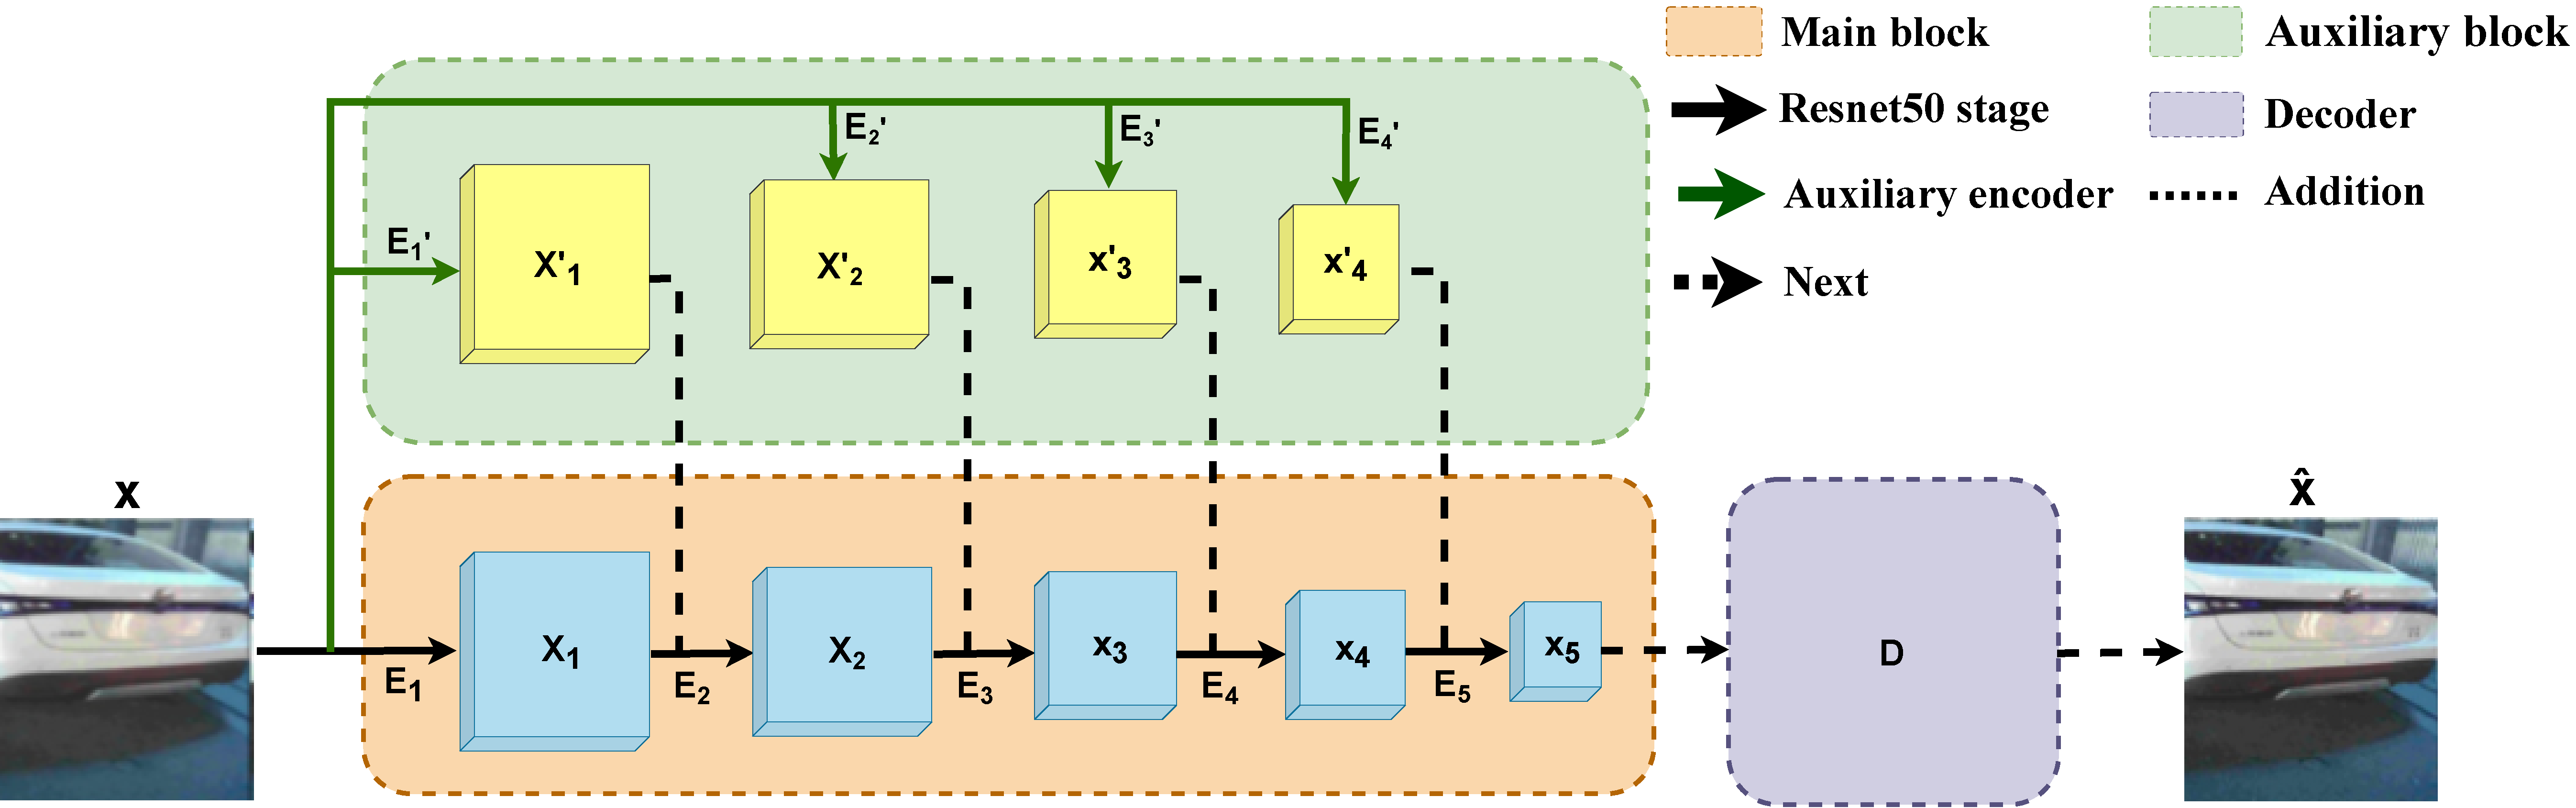
\includegraphics[width=0.9\linewidth]{images/VRAE.pdf}
                \caption{Kiến trúc VRAE}
            \end{figure}
        \end{column}
    \end{columns}
\end{frame}

\begin{frame}{Khối chính (Main Block)}
    \begin{columns}
        \begin{column}{0.4\textwidth}
            \textbf{Cấu trúc:}
            \begin{itemize}
                \item Dựa trên ResNet-50 (Stage 1-5)
                \item Cấu trúc Bottleneck:
                \begin{itemize}
                    \item $1 \times 1$: Giảm chiều
                    \item $3 \times 3$: Xử lý không gian
                    \item $1 \times 1$: Khôi phục kênh
                \end{itemize}
                \item Skip-connection: Cải thiện gradient flow
            \end{itemize}
        \end{column}
        \begin{column}{0.5\textwidth}
            \textbf{Kết nối dọc:}
            \begin{equation}
                \mathbf{x}_i = E_i(\mathbf{x}_{i-1} + \mathbf{x}'_{i-1})
            \end{equation}
            \begin{itemize}
                \item $\mathbf{x}_{i-1}$: Đầu ra khối chính
                \item $\mathbf{x}'_{i-1}$: Đầu ra khối bổ trợ
                \item Hội tụ đặc trưng đa cấp
            \end{itemize}
        \end{column}
    \end{columns}
\end{frame}

% \subsection{Khối bổ trợ}
\begin{frame}{Khối bổ trợ (Auxiliary Block)}
    \textbf{Mục đích:} Tăng cường khả năng giữ lại thông tin cục bộ và ngữ cảnh
    
    \vspace{0.3cm}
    \begin{columns}
        \begin{column}{0.5\textwidth}
            \textbf{Đặc điểm:}
            \begin{itemize}
                \item Cấu trúc Conv-Norm-Activation
                \item Trích xuất đặc trưng trực tiếp từ ảnh gốc:
                \[
                    \mathbf{x}'_i = E'_i(\mathbf{x}), \quad i = 1, \dots, 5
                \]
            \end{itemize}
        \end{column}
        \begin{column}{0.5\textwidth}
            \textbf{Lợi ích:}
            \begin{itemize}
                \item Làm giàu biểu diễn low/mid-level
                \item Bổ sung manh mối trực tiếp từ ảnh gốc
                \item Giúp bảo toàn chi tiết tần số cao
                \item Tăng số tham số không đáng kể so với tăng độ sâu mô hình
            \end{itemize}
        \end{column}
    \end{columns}
\end{frame}

% \subsection{Bộ giải mã}
\begin{frame}{Bộ giải mã (Decoder)}
    \textbf{Nhiệm vụ:} Khôi phục ảnh từ biểu diễn nén
    
    \vspace{0.3cm}
    Quá trình lấy mẫu lên (upsampling):
    \begin{equation}
        \mathbf{y}_k = \text{ReLU}(\text{ConvTranspose2d}_k(\mathbf{y}_{k-1}))
    \end{equation}
    với $k=1, \dots, 5$, $\mathbf{y}_0 = \mathbf{x}_N$, $\mathbf{y}_K = \hat{\mathbf{x}}$
    
    \vspace{0.3cm}
    \textbf{Hàm mất mát:}
    \begin{equation}
        \mathcal{L}_{\text{MSE}} = \frac{1}{BCHW} \sum_{b,c,i,j} (\hat{x}_{b,c,i,j} - x_{b,c,i,j})^2
    \end{equation}
    
    \begin{itemize}
        \item Đơn giản, ổn định
        \item Phù hợp với mục tiêu khôi phục độ trung thực tín hiệu (PSNR)
        \item Tối ưu hóa trực tiếp sai số tái cấu trúc
    \end{itemize}
\end{frame}

\begin{frame}{Chuẩn bị dữ liệu và huấn luyện}
    \begin{columns}
        \begin{column}{0.5\textwidth}
            \textbf{Dữ liệu:}
            \begin{itemize}
                \item CCPP Dataset: 3,036 ảnh gốc
                \item Kích thước: $256 \times 256$ pixels
                \item Phân chia: 70\%-15\%-15\%
                \item Data augmentation: $\rightarrow$ 7,000 ảnh train
            \end{itemize}
            
            \vspace{0.3cm}
            \textbf{Mô phỏng suy giảm:}
            \begin{itemize}
                \item Nhiễu rời rạc (0-9, nhân 0.1)
                \item Average pooling $3 \times 3$ (10 lần)
            \end{itemize}
        \end{column}
        \begin{column}{0.5\textwidth}
            \textbf{Cấu hình huấn luyện:}
            \begin{itemize}
                \item Optimizer: Adam
                \item Learning rate: $1 \times 10^{-4}$
                \item Batch size: 16
                \item Epochs: 100
                \item GPU: NVIDIA RTX 4070
            \end{itemize}
            
            \vspace{0.3cm}
            \textbf{So sánh với:}
            \begin{itemize}
                \item AE (2-5 stages)
                \item GAN
                \item Flow-based (FB)
            \end{itemize}
        \end{column}
    \end{columns}
\end{frame}

